\subsection{Rolling Cadence} \label{q:Rolling}

The Phase 1 SCOC report included a recommendation to adopt a half-sky rolling cadence and to continue to investigate rolling options. With the expansion of the footprint recommended in Phase 1 (see \autoref{q:Footprint}), the number of visits per pointing in the WFD dropped slightly, with an associated impact on metrics dependent on cadence in the few days range. The inclusion of rolling in the cadence, which concentrates visits into some region of sky during some seasons at the expense of visits' cadence during other seasons, was intended to counter this drop in cadence near the 3-5 day range (see \citetalias{PSTN-053} Q6).


The questions left open after the Phase 1 recommendations on rolling cadences were: 

\begin{enumerate}
\item Should a rolling cadence be adopted in the WFD?
\item Should a rolling cadence be adopted in the special regions of the WFD (NES, GP, SCP) and minisurveys?
\item Which scheme for rolling should be adopted? (number of rolling regions, other spatial region splits)
\item How aggressive should the strength of the rolling be in the WFD or non-WFD footprint?
\item When should rolling start (end of year 1 or after 1.5 years)?
\end{enumerate}

\subsubsection{SCOC recommendations: executive summary}\label{sec:rolling}

 The SCOC reviewed metrics from the community, especially as presented in notebooks that compared the performance across v2.X simulations and earlier baselines.\footnote{See: \url{https://github.com/lsst-pst/survey_strategy/blob/main/fbs_2.0/Rolling\%20Cadence.ipynb} and \url{https://github.com/lsst-pst/survey_strategy/blob/main/fbs_2.0/Rolling\%20Cadence\%20v2.2.ipynb}.} Following the Phase 1 SCOC recommendations, rolling is implemented as a default in v2.X simulations with a split into two half-sky regions defined by declination limits and with a $\sim0.9$ rolling weight\footnote{The weight is the relative fractions of images that the scheduler is requested to schedule on the active \emph{vs} inactive regions of sky. However, it should be noted that additional constraints on the number of images (\emph{e.g.}, collection of a sufficient number of images over time to enable the creation of templates) are likely to cause the number of images actually collected to differ from this request.} \citepalias{PSTN-051}. {\bf While some details remain to be optimized jointly with other SCOC choices, the SCOC recommendation is for a half-sky 0.9-weight rolling cadence on the WFD and, tentatively, on the Galactic Plane and Bulge as well, as a practical compromise to support both static-sky science and time-varying science.    
This recommendation is made under the assumption that sufficient uniformity in depth to support static-sky cosmology (and more in general, static-sky science) in annual data releases can be achieved in data-processing.  Should this not be the case, the SCOC will re-evaluate this recommendation.}


 \begin{figure}
    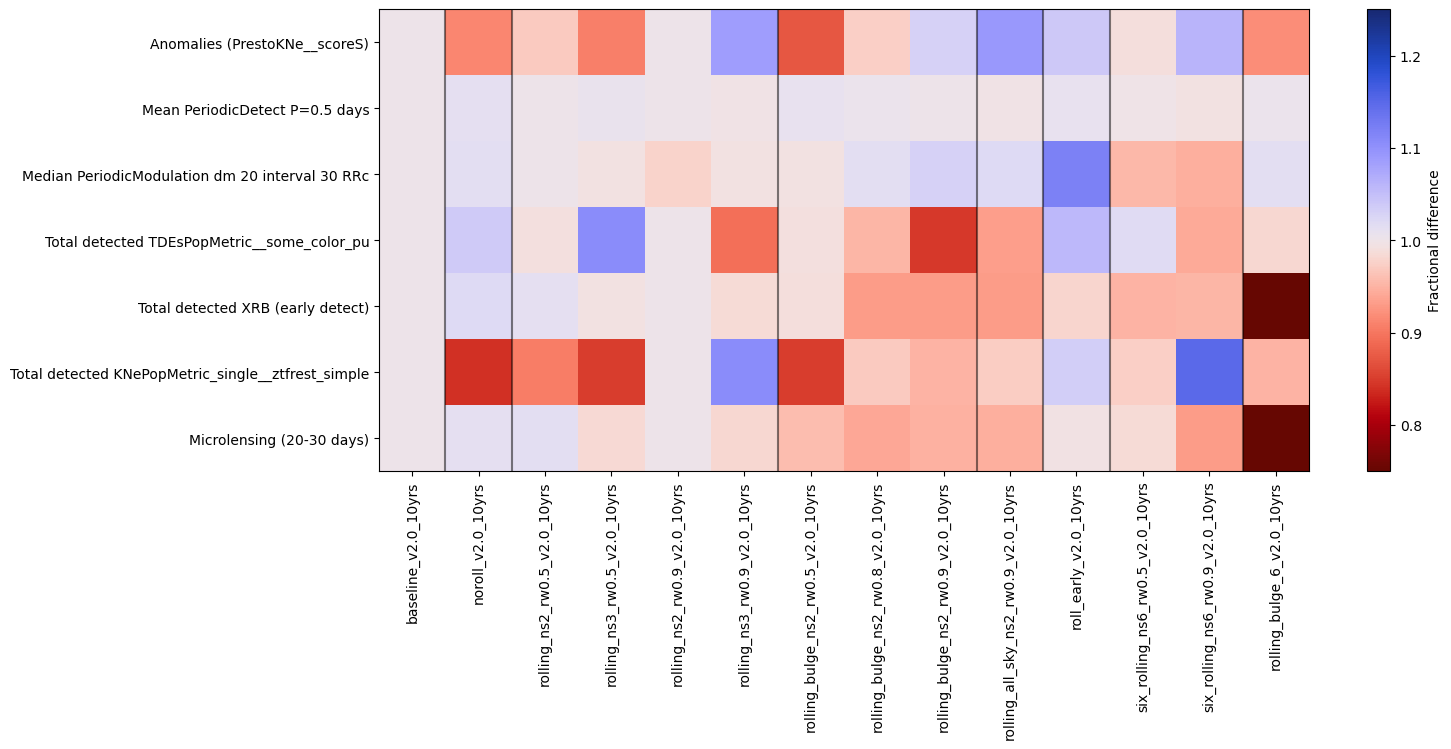
\includegraphics[width=\textwidth, right]{figures/roll_tvs.png}
     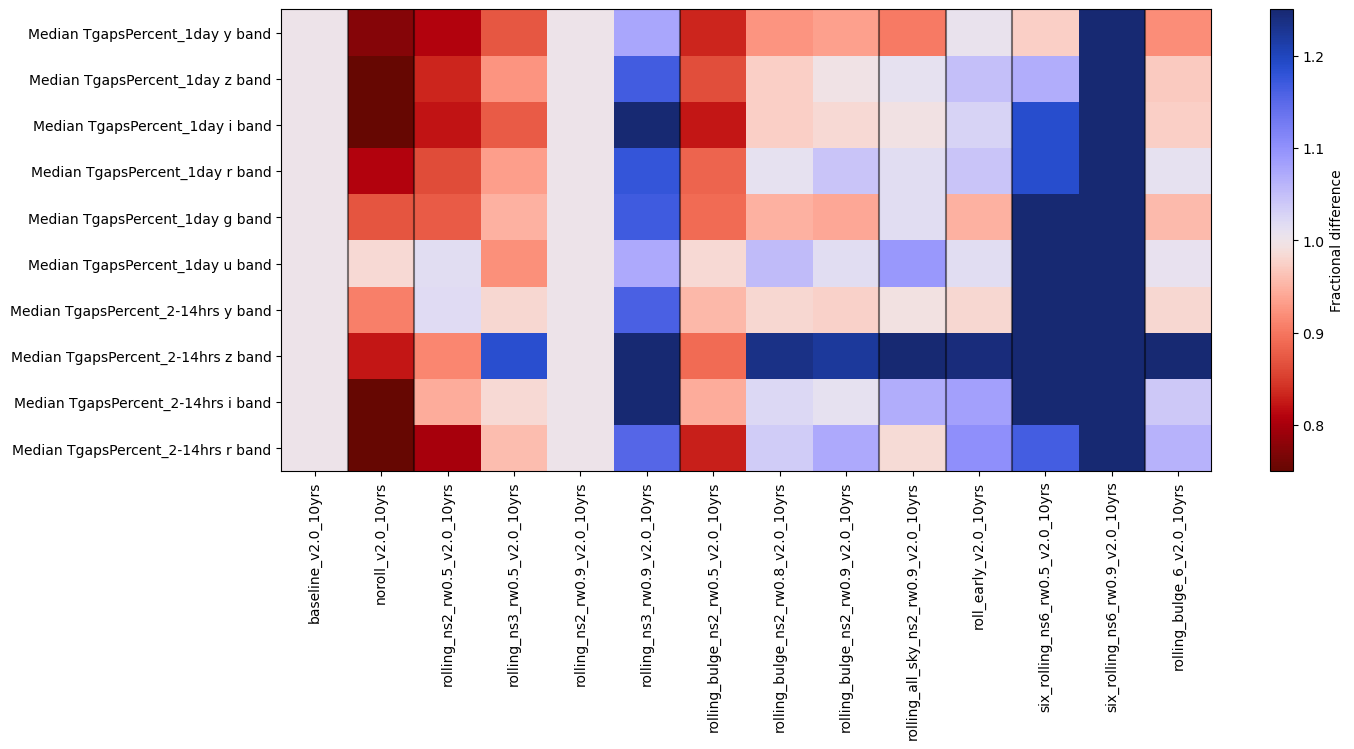
\includegraphics[width=0.93\textwidth, right]{figures/roll_tgaps.png}\caption{Some of the metrics considered in deliberating about a rolling strategy for LSST and their performance for selected 2.0 simulations (the reference simulation for both plots being \texttt{baseline\_v2.0}, which implements half-sky rolling at 0.9 weight). Top: time-domain metrics. While time-domain metrics that monitor long transients (e.g. TDE) prefer weak or no rolling, rapid transients strongly prefer rolling (kilonovae and anomalies metrics). This is because of the additional coverage on time scales $<2$ days, as seen in the bottom panel which shows the percentage of observations following in specific time scales with specific filters. However, very aggressive rolling, for example in 6 sky areas (\texttt{\_ns6\_}), is strongly disfavored by many time-domain metrics because of the reduced survey efficiency due to additional constraints on pointing.}
     \label{fig:knroll}
 \end{figure}

 \subsubsection{SCOC recommendations: point by point answers}\label{sec:rolling_points}
 


\begin{enumerate}
    \item 
The SCOC supports a rolling cadence\footnote{A cadence where a portion of the sky is emphasized in one rolling cycle, to then be de-emphasized in the following rolling cycles.} and recommends that rolling be adopted across the WFD. Our recommendation is based on the review of the metrics and reports from all SCs. Transient metrics for the extragalactic sky strongly support rolling. A non-rolling cadence would negatively affect all extragalactic transient metrics presented by TVS, typically by 20\%.
 The DESC supports a rolling cadence as it is shown to improve the sampling of SN Ia light curves for cosmological characterization (see Sec 9.5 and Fig 9.22 of \citealt{cosep} and \citealt{https://doi.org/10.48550/arxiv.2210.15690}). The SSSC and AGN SC metrics perform well or neutrally with some rolling, although the strength of rolling has to be decided carefully, and we return to this point in our response to points 3 and 4. 
 
 \item \emph{The SCOC does not have a final recommendation for rolling on the Galactic Plane/Bulge at this time}. The decision about rolling in this area is compartmentalized and should not impact the WFD performance, though this assumption has to be verified via simulations. Thus the SCOC can continue to optimize the rolling choices on the Galactic Plane, together with the details on the filter balance and footprint over the Galactic Plane (\autoref{q:Footprint} and \autoref{q:Filters}). The current implementation of rolling on the Galactic Plane with the same scheme adopted in the WFD seems, however, to be a good compromise to support short- and long-variability phenomena (see below). No simulations with rolling on the NES and SCP or minisurveys have been created to date. The NES and SCP have fewer visits and may therefore not benefit from rolling, and it may not even be possible to implement rolling while also producing adequate annual templates. 

 \item Questions 3 and 4 will be discussed jointly: 
 
 \item The decision about the strength of rolling concerns both the number of areas over which rolling occurs and the weight of the rolling (the fraction of the time spent on the on \emph{vs} off sky regions).  The SCOC has reviewed combinations of rolling implemented on sky splits into 6 rolling regions, 3 rolling regions, and 2 rolling regions (or half-sky) and at 0.5, 0.8, and 0.9 rolling weight in v2.X simulations. When analyzing the strength of a rolling cadence, in the segmentation of the sky or in the rolling weight, SCOC considerations, guided by the community metrics, include the impact on transient phenomena characterization at all time scales (\autoref{fig:knroll}), but also the impact on the uniformity of the data releases in terms of coverage and depth (\autoref{fig:rolluniformity}). In particular: the DESC science requires a certain degree of uniformity in intermediate data releases for static sky cosmology and the DESC urged, via its reports\footnote{\label{fn:descreport}\url{https://lsst.org/sites/default/files/documents/DESC-SCOC_November2022.pdf}} and its liaisons, that Rubin intermediate data products (galaxy catalogs, etc.) be made from as uniform-depth extragalactic WFD data as possible. This is likely to be a concern for other static-sky science as well, such as the science relevant to the Galaxies SC and Strong Lensing SC. \emph{A measurable definition of the required uniformity and evaluations of the data processing options to achieve it should be undertaken in 2023}. AGN metrics for detecting Blazar time lags are insensitive to rolling cadence but can underperform if objects are poorly characterized due to the long gaps in coverage, which would happen in the off-sky regions for aggressive rolling patterns. The AGN Structure Function metric also sees an increase in errors with 6 sky areas identified for rolling (``6-band'' rolling). Finally, with such high sky segmentation, slow-evolving transients would be poorly characterized (although most transient metrics focus on fast transients and early transient characterization and may not reflect this concern). In addition, adding constraints on the pointing reduces the efficiency of the survey by reducing the ability to select a position on the sky that minimizes slew and that maximizes image quality. Thus most metrics, including time-domain metrics, suffer when aggressive rolling schemes with high sky segmentation are implemented (\emph{e.g.} in sky sixths, or ``6-band'' rolling) because of the overall reduced number of images and survey depth. Therefore, the SCOC overall disfavors an aggressive ``6-band'' rolling cadence.
 \begin{figure}
    \centering
    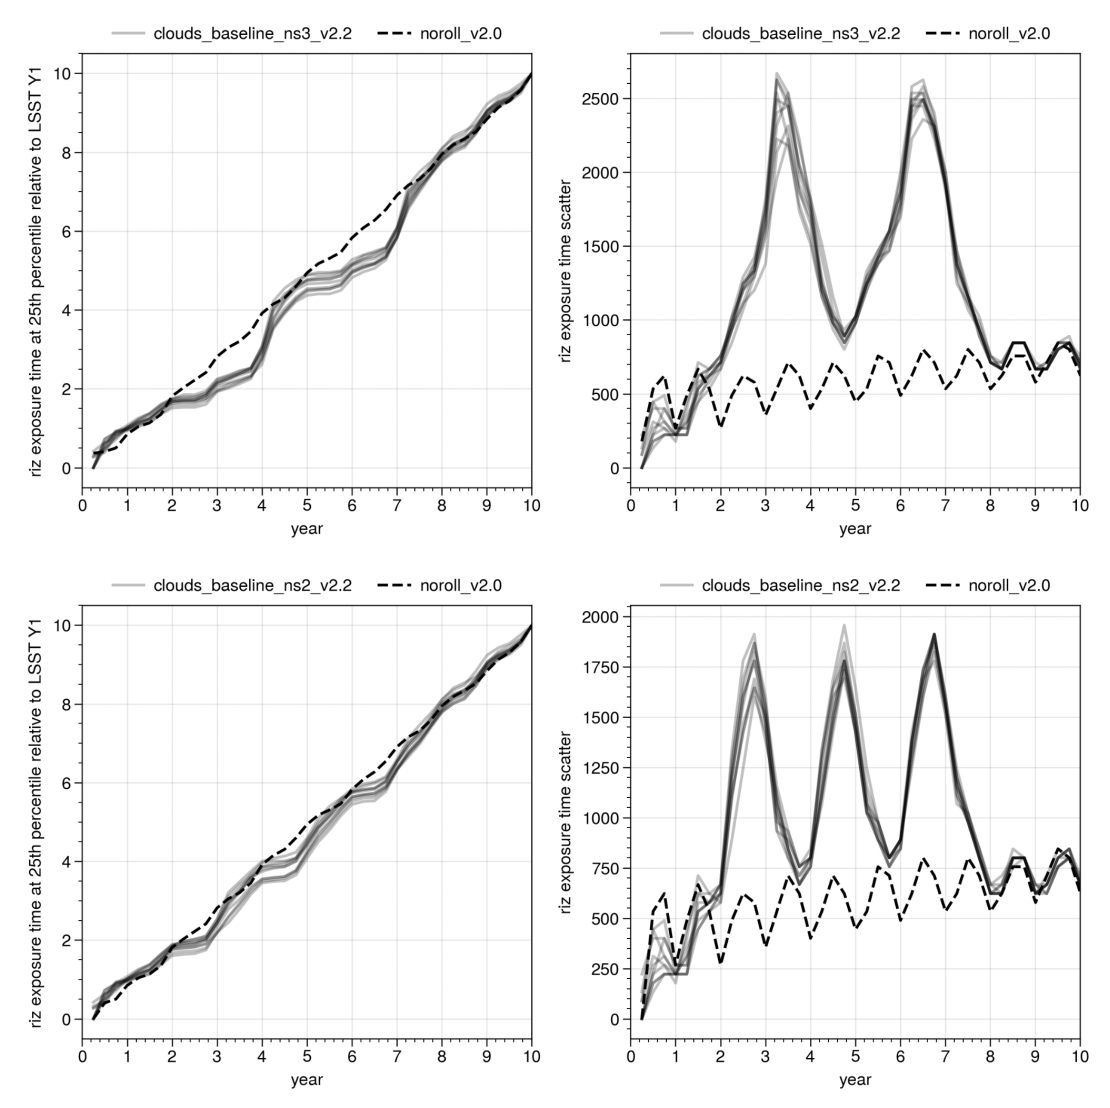
\includegraphics[width=0.6\textwidth]{figures/uniformity_DESC.png}
     
     \caption{Uniformity of annual data releases (produced by M. Becker, DESC${fn:descreport}$
     )
     : \emph{Left}: cumulative exposure time per sky region relative to year 1; \emph{right}: scatter in the exposure time.
     Rolling cadences in sky thirds (\texttt{cloud\_baseline\_ns3\_v2.2}, \emph{top}) and half-sky rolling (\texttt{cloud\_baseline\_ns2\_v2.2}, \emph{bottom}) with a 0.9 weight, where rolling begins after year 1, shown against a non-rolling simulations (dashed line). The rolling strategies are shown for multiple simulations with varying cloud patterns. Rolling over half the sky has a significant impact on the uniformity needed for static science in years ~3, 5, and 7, but recovers in years 4, 6, and 8. A rolling scenario with sky segmentated into thirds (sometimes referred to as ``3-band'' rolling) causes significant degradation in uniformity over years 3, 4, 6, and 7, and the recovery of uniformity by year 5 is not as complete as in the half-sky case. }
     \label{fig:rolluniformity}
 \end{figure}

  While splitting the sky into thirds (earlier referred to as ``3-band'' rolling scheme) and rolling at a 0.9 weight would produce a good sampling of transients, including fast transients such as kilonovae by covering short time scales (see Kilonova metrics, \autoref{fig:knroll}, top), it would negatively impact metrics measuring data release uniformity (see the November 2022 DESC report\footnote{\url{https://lsst.org/sites/default/files/documents/DESC-SCOC_November2022.pdf}} and \autoref{fig:rolluniformity}) and Strong Lensing metrics. Conversely, a half-sky 0.9 weight rolling strategy \emph{alone} would leave time scales between 2-14 hours and one day undersampled and unexplored, with decreased performance on fast transients and potential loss of discovery (\autoref{fig:knroll}, bottom). However, as discussed in \autoref{q:Visits}, choices that control the intra- and inter-night cadence could solve the hour-to-one-day time scale issues and be jointly applied with rolling to achieve optimal results.  %To confirm that this is indeed optimal, we require a few simulations to be produced explicitly tuning these parameters.  
  The current SCOC recommendation is for half-sky rolling and 0.9 rolling weight. The optimization of rolling parameters is intertwined with the choice of intra-night cadence and repeat observations and triplets every few to several days and observations on the following day performed often in combination with this rolling scheme are likely to achieve the desired results. Note that in a half-sky rolling scheme the sky is actually split into 4 regions defined by declination, of which two are active at a given time (see \autoref{sec:v3}). 
  
  The new baseline represents a significant relative improvement over previous implementations of a rolling cadence but further refinement could help boost the low absolute numbers of visits in underexplored and poorly explored times scales. Therefore, this recommendation should not be interpreted as final; joint optimization of the observation repeat pattern and rolling should be continued by the SCOC. 

  \item Rolling should start after the first part of the sky which has had a complete season of observations
in “uniform” cadence starts its second season. That is roughly 1.5 years after the start of the survey. Early rolling (\emph{e.g.}, starting at or near the end of year 1) would lead to severe non-uniformity that would compromise DESC early science.${fn:descreport}$

\end{enumerate}
